% Material found at https://www.elsevier.com/authors/author-schemas/latex-instructions

\documentclass{elsarticle}

\usepackage{lineno,hyperref}
\modulolinenumbers[5]

%=== Added for MU paper ====
\usepackage{color,soul} %% this was needed to have highlighted text
\usepackage{graphicx}
\usepackage{array,colortbl,xcolor}
\usepackage{hyperref}
\usepackage{amsmath}
\usepackage{amssymb}
\usepackage{mathtools}
\usepackage{nomencl}
\usepackage{bm}
\usepackage{subcaption}
\usepackage{systeme}
\makenomenclature

\graphicspath{{./figures/}}

\renewcommand{\labelenumii}{\theenumii}
\renewcommand{\theenumii}{\theenumi.\arabic{enumii}.}

\journal{Reliability Engineering \& System Safety}

%%%%%%%%%%%%%%%%%%%%%%%
%% Elsevier bibliography styles
%%%%%%%%%%%%%%%%%%%%%%%
%% To change the style, put a % in front of the second line of the current style and
%% remove the % from the second line of the style you would like to use.
%%%%%%%%%%%%%%%%%%%%%%%

%% Numbered
\bibliographystyle{model1-num-names}

%% Numbered without titles
%\bibliographystyle{model1a-num-names}

%% Harvard
%\bibliographystyle{model2-names.bst}\biboptions{authoryear}

%% Vancouver numbered
%\usepackage{numcompress}\bibliographystyle{model3-num-names}

%% Vancouver name/year
%\usepackage{numcompress}\bibliographystyle{model4-names}\biboptions{authoryear}

%% APA style
%\bibliographystyle{model5-names}\biboptions{authoryear}

%% AMA style
%\usepackage{numcompress}\bibliographystyle{model6-num-names}

%% `Elsevier LaTeX' style
%\bibliographystyle{elsarticle-num}
%%%%%%%%%%%%%%%%%%%%%%%

\begin{document}

\begin{frontmatter}

\title{Measuring Risk-Importance in a Simulation-Based PRA Framework - 
       Part II: Comparison with Classical PRA Methods}
%% \tnotetext[mytitlenote]{Fully documented templates are available in the elsarticle package on \href{http://www.ctan.org/tex-archive/macros/latex/contrib/elsarticle}{CTAN}.}

%% Group authors per affiliation:
\author{D. Mandelli, C. Parisi, Z. Ma, D. Maljovec, C. Smith}
\address{Idaho National Laboratory (INL), 2525 Fremont Ave, 83402 Idaho Falls (ID), USA}

\begin{abstract}
  Risk importance measures are indexes that are used to rank systems, 
structures and components (SSCs) using risk-informed methods. 
The most used/known measures are: Risk Reduction Worth (RRW), 
Risk Achievement Worth (RAW), Birnbaum (B) and Fussell-Vesely (FV). 
Once obtained from classical Probabilistic Risk Analysis (PRA) analyses, 
these risk measures can be effectively employed to relatively rank
component importance.
In contrast to classical PRA methods, 
Dynamic PRA methods couple stochastic models with safety analysis 
codes to determine risk associate to complex systems such as nuclear 
plants. Compared to classical PRA methods, simulation-based approaches
can evaluate with 
higher resolution the safety impact of timing and sequencing of events 
on the accident progression. 
The objective of this paper is to present a series of methods that 
can be employed to measure risk importance of components which are 
part of complex systems such as nuclear power plants.
The first set of measures are directly derived from classical risk 
importance measures (e.g., RRW, RAW, B and FV) and that can be employed
to any Dynamic PRA analysis.
In addition, we provide a set of risk importance measures that capture the 
dynamic nature of the problem and provide insight related to plant safety 
margins.

\end{abstract}

\begin{keyword}
%% keywords here, in the form: keyword \sep keyword
Importance Measures \sep Dynamic PRA \sep Probabilistic Risk Assessment 
\end{keyword}

\end{frontmatter}

\linenumbers

\printnomenclature[1in]

\section{Introduction}
\label{sec:introduction}
RAVEN (\textbf{R}isk \textbf{A}nalysis \textbf{V}irtual \textbf{EN}vironment)~\cite{Nureg1150}  is one of the many INL-developed software tools researchers can 
use to identify and 
increase the safety margin in complex systems (e.g. Nuclear Power Plants). It is a modular or ``plug-able'' framework that can be coupled with other computer 
modeling systems. RAVEN is capable to agnostically communicate with any system 
code. This agnosticism includes providing Application Programming Interfaces (APIs). These APIs are used to allow RAVEN to interact with any code as long as all 
the parameters that need to be perturbed are accessible through input files or via python interfaces. 
As a generic software framework, RAVEN is designed to perform parametric and probabilistic analysis based on the response of complex system codes. RAVEN is 
capable of investigating the system response as well as the input space using standard sampling techniques (e.g Monte Carlo, Grid, or Latin Hyper Cube), but its 
strength is focused toward system feature discovery, such as limit surfaces (i.e. separating regions of the input space leading to system failure, using dynamic 
supervised learning techniques), and advanced data analysis methodologies (i.e. Topology-based domain decomposition, Data Mining, Clustering, etc.).

The development of RAVEN has begun in 2012 to satisfy the need to provide a modern risk evaluation framework. RAVEN principal assignment is to provide the 
necessary software and algorithms in order to employ the concept developed by the Risk Informed Safety Margin Characterization (RISMC) path-
way~\cite{RISMC}. 
RISMC is one of the pathways defined within the Light Water Reactor Sustainability (LWRS) program. In the RISMC approach, the goal is not just specifically 
identifying the frequency of an event potentially leading to a system failure, but also to analyze the ``distance'' and the drivers toward the happening of key 
safety-related events. This approach may be used in identifying and increasing the safety margins related to those events. A safety margin is a numerical value 
quantifying the probability that a safety metric (e.g. as peak pressure in a pipe) is exceeded under certain conditions. The initial development of RAVEN has 
been focused on providing dynamic risk assessment capability to RELAP-7~\cite{RELAP7}, currently under development at the INL. All the methodologies
developed have been modularized in order to be applied to any computer modeling system (e.g., BISON, RELAP-7, RELAP5-3D, MELCOR, etc.).

The aim of this manuscript is to present a peculiar capability within the RAVEN framework named \textit{``EnsembleModels''}.

RAVEN is currently able to construct multi-targets Reduced Order Models (Ref.4), which are aimed to represent the response of a system (in a 
fixed configuration) for multiple Figures of Merits (FOMs) and time-dependent ROMs (see Ref.5). These capabilities represent the initial steps for a larger 
implementation about the interaction of multiple models. In fact, in several cases, multiple models need to interface with each other since the initial conditions of 
one are dependent on the outcomes of another.
To better understand the problem that here is solved, it is useful to consider two simple examples:
\begin{enumerate}
  \item The following problem is considered: a weather forecast simulation code ``a'' is used to compute the external (i.e. ambient) temperature in a certain location. 
  A second model ``b'' is inquired to compute the average temperature in a room having as boundary condition, among several others, the external ambient 
  temperature. The response of the model ``b'' depends on the outcome of the model ``a'';
   \item Two different simulation codes are considered: a) a code that is meant to compute the thermal conductivity of the ceramic Uranium Dioxide (UO2) as 
   function of the Temperature, and b) a Thermal-hydraulic (TH) code that is used to compute the Temperature field of a reactor, whose heat conduction depends on 
   the thermal conductivity value. As easily inferable, the two models are mutual dependent, determining in a non-linear system of equations.
\end{enumerate}
The two reported examples are only aimed to illustrate the reason why the creation of a framework to make interact different models is a key development for the 
advancement of RAVEN as a comprehensive calculation flow driver. Before reporting how the ensemble-models have been implemented, it is necessary to briefly 
describe the representative Model ``entities'' that are available in RAVEN.



\begin{figure}
    \centering
    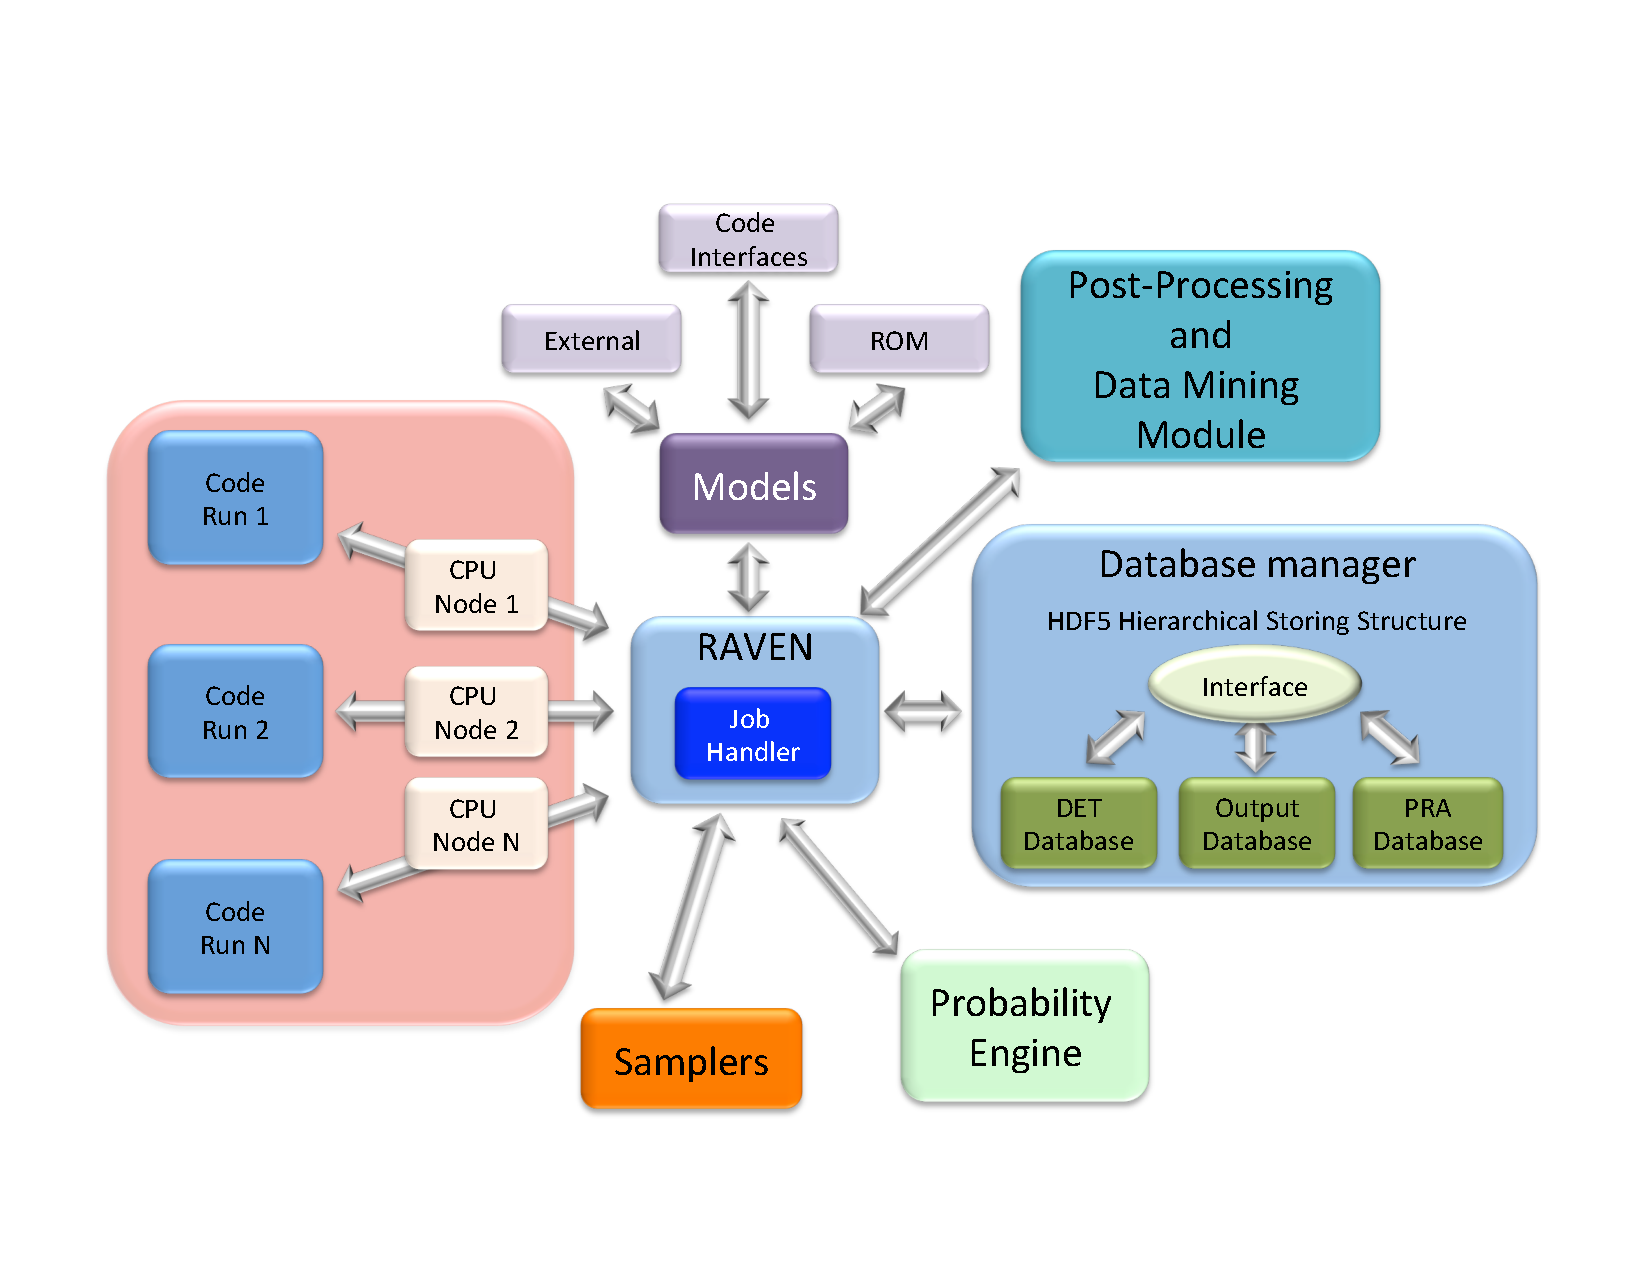
\includegraphics[scale=0.5]{raven.pdf}
    \caption{RAVEN}
    \label{fig:raven}
\end{figure}

\section{Comparison}
\label{sec:comparison}

[text]
\section{SAPHIRE modeling [zhegang]}
\label{sec:SAPHIREmodeling}

[text]

\subsection{ET-FT reformulation [zhegang]}

[text]
\section{PWR Deterministic Modelling}
\label{sec:PWRdeterministicModeling}

SAPHIRE code Standardized Plan Analysis Risk (SPAR) used for static PRA analysis is based on a generic 3-loops Westinghouse PWR model. Dynamic PRA calculations were executed by RELAP5-3D/RAVEN, so a RELAP5-3D system code model for a generic 3-loops Westinghouse PWR has been developed. The description of this model is reported hereafter.


\subsection{RELAP5-3D Model for 3 Loops PWR}

The RELAP5-3D model is based on the so-called INL Generic PWR (IGPWR) model used for calculations of different LWRS/RISMC tasks. 
The RELAP5-3D input deck is modeling a ~2.5 GWth Westinghouse 3-loops PWR, including the reactor pressure vessel (RPV), the 3 loops and the primary and secondary sides of the steam generators (SG) (see Figure~\ref{fig:rpv} and Figure~\ref{fig:mcc}).  

\begin{figure}
    \centering
    \includegraphics[scale=0.9]{RPV.png}
    \caption{RELAP5-3D RPV Model.}
    \label{fig:rpv}
\end{figure} 

\begin{figure}
    \centering
    \includegraphics[scale=0.9]{MCC.png}
    \caption{RELAP5-3D MCC and SG Model.}
    \label{fig:mcc}
\end{figure} 

Four independent channels are used for representing the reactor core. Three channels model the active core and one channel models the core bypass. Different power values are assigned to the three core channels in order to take into account the radial power distribution. Passive and active heat structures simulate the heat transfer between the coolant and fuel, the structures and the secondary side of the IGPWR.

\begin{figure}
    \centering
    \includegraphics[scale=1.0]{CORE_POW.png}
    \caption{RELAP5-3D Core Model.}
    \label{fig:CORE_POW}
\end{figure} 

Table~\ref{tab:dataRelap5} reports the steady state values obtained for the RELAP5-3D model and the comparison with reference values, showing that the agreement is good. 

\begin{table}
  \centering
  \begin{tabular}{c | c | c | c} 
    \hline 
     Parameter & Reference value & RELAP5-3D value & Deviation (\%) \\
    \hline 
     Reactor Power (W) & 2,546 & 2,546 & imposed \\
     PRZ Pressure (MPa) & 15.5 & 15.57 & imposed \\
     Total RCS Coolant Loop Flowrate (Kg/s) & 12,738 & 12,738 & 0.0 \\
     CL Temperature (K) & 555.6 & 557.3 & 0.3 \\
     HL Temperature (K) & 591.8 & 593.1 & 0.2 \\
     Feed-water Temperature (K) & 501.5 & 501.5 & imposed \\
     Steam Flowrate per SG1 (K) & 473. & 470.1 & -0.6 \\
     Steam Flowrate per SG2 (K) & 473. & 470.7 & -0.5 \\
     Steam Flowrate per SG3 (K) & 473. & 471.0 & -0.4 \\
     Steam Pressure at the Outlet Nozzle (MPa) & 5.405 & 5.405 & imposed \\
     Liquid Mass per SG (Kg) & 41,639 & 41,640 & 0.0 \\
     Steam Temperature (K) & 542 & 542 & 0.0 \\
    \hline 
  \end{tabular}
  \caption{RELAP5-3D LBLOCA steady state values.}
  \label{tab:dataRelap5}
\end{table}

For the transient calculation, a horizontal LBLOCA on the cold-leg RPV nozzle was considered. The break was supposed to happen on the pressurizer loop. Several LBLOCA cases were run, including some considered by Westinghouse for LBLOCA spectrum analysis (U.S. NRC 2011):
\begin{itemize}
	\item 2A, Double-Ended Guillotine Break (DEGB);
	\item 1A;
	\item 10 inches diameter;
	\item 8 inches diameter;
	\item 6 inches diameter.
\end{itemize}

For the LBLOCA DEGB, the total break area was 2x0.383 m2 (2x4.125 ft2), corresponding to a 0.7 m (27.56 inches) diameter pipe. The RELAP5-3D model of the break is reported in Figure~\ref{fig:debg}. 

\begin{figure}
    \centering
    \includegraphics[scale=0.6]{DEGB.png}
    \caption{RELAP5-3D LBLOCA DEGB model scheme.}
    \label{fig:debg}
\end{figure} 

For the other 4 cases, the total break area was:
\begin{itemize}
	\item case 1A: 0.383 m2 (4.125 ft2), or 0.7 m (27.5 inches) diameter break;
	\item case 10 inches: 0.0506 m2 (0.545 ft2), or 0.254 m (10 inches) diameter break;
	\item case 8 inches: 0.0324 m2 (0.349 ft2), or 0.203 m (8 inches) diameter break;
	\item case 6 inches: 0.0182 m2 (0.196 ft2), or 0.152 m (6 inches) diameter break.
\end{itemize}

The scheme of the break is reported in Figure 5.

\begin{figure}
    \centering
    \includegraphics[scale=0.6]{1AandOthers.png}
    \caption{RELAP5-3D LBLOCA 1A/10-8-6 inches model scheme.}
    \label{fig:1AandOthers}
\end{figure} 

The Emergency Core Cooling Injection System (ECCS) model is based on the information provided by (U.S. NRC 2011), (NRC 2013), (Dominion 2007). The main characteristics of it are reported in Table~\ref{tab:dataRelap5_ECCS}, Table~\ref{tab:dataRelap5_RWST} and Table~\ref{tab:dataRelap5_cont}. 

\begin{table}
  \caption{RELAP5-3D ECCS main parameters.}
  \centering
  \begin{tabular}{c | c | c} 
    \hline 
     ECCS Parameters & Value (SI) & Value (Imperial) \\
    \hline 
    Accumulator Water Volume [m3 / ft3] & 3 x 28.32 & 3 x 1000 \\
    Accumulator Gas Pressure [MPa / psig] & 4.00 & 580 \\
    Accumulator Water Temperature [C / F] & 40.6 & 105.0 \\
    HPI volumetric flow [m3/s /gpm] & 3 x 0.0708 (at 1,767 m) & 3 x 150 (at 5,800 ft) \\
    HPI design head [MPa / psi] & 17.34 & 2515.3 \\
    LPI volumetric flow [m3/s /gpm] & 2 x 1.416 (at 68.6 m) & 2 x 3,0007 (at 225 ft) \\
    LPI design head [MPa / psi] & 6.728 & 97.58 \\
    \hline 
  \end{tabular}
  \label{tab:dataRelap5_ECCS}
\end{table}

\begin{table}
  \caption{RWST main parameters.}
  \centering
  \begin{tabular}{c | c | c} 
    \hline 
    Parameters & Value (SI) & Value (Imperial) \\
    \hline 
    Max Water Volume [m3 / gal] & 1514.2 & 400,000 \\
    Required Minimum Water Volume [m3 / gal] & 1465.3 & 387,000 \\
    Minimum Water Volume  [m3 / gal] & 53.0 & 14,000 \\
    Water Temperature [C / F] & 7.2 & 45.0\\
    RWST / Containment sump switch time (s) & 150.0 & \\
    \hline 
  \end{tabular}
  \label{tab:dataRelap5_RWST}
\end{table}

\begin{table}
  \caption{Containment main parameters.}
  \centering
  \begin{tabular}{c | c | c} 
    \hline 
    Parameters & Value (SI) & Value (Imperial) \\
    \hline 
    Volume [m3 / ft3] & 49,000 & 1,730,000 \\
    Design Pressure [MPa /psig] & 0.31 & 45 \\
    Operating Pressure [MPa /psia] & 0.062 to 0.071 & 9 to 10.3 \\
    Operating Temperature [C / F] & 24 to 52 & 75 to 125 \\
    Containment sprays mass flow [m3/s /gpm] & 2 x 0.183 & 2 x 2900 \\
    \hline 
  \end{tabular}
  \label{tab:dataRelap5_cont}
\end{table}

The actuation signals for the ECCS and the containment sprays are reported in Table~\ref{tab:dataRelap5_signals}.

\begin{table}
  \caption{ECCS and Containment Spray actuation signals.}
  \centering
  \begin{tabular}{c | c | c} 
    \hline 
    Parameters & Value (SI) & Value (Imperial) \\
    \hline 
    Low pressure signal in PRZ [MPa/psig]  & $<12.3$ & $<1789.7$ \\
    Low-low pressure signal in PRZ [MPa/psig] & $<12.2$ & $<1775.$ \\
    High Containment Pressure [MPa/psia] & $>0.122$ & $>17.7$ \\
    High Steamline Delta Pressure [MPa/psid] & $>0.827$ & $>120.$ \\
    Spray signal for Containment Pressure [MPa/psig] & $>0.172$ & $>25$ \\
    Spray OFF for Containment Pressure [MPa/psig] & $<0.082$ & $<12$ \\
    \hline 
  \end{tabular}
  \label{tab:dataRelap5_signals}
\end{table}

The operators and the emergency crew actions were limited to few actions. The initial ECCS and containment sprays actuations were supposed to be automatically performed by the reactor protection system. 


\section{PWR Stochastic Modeling}
\label{PWRstochasticModeling}

[text]
\section{ROM modeling}
\label{sec:ROMmodeling}

[text]
\section{RISMC results}
\label{sec:RISMCresults}

[text]
\section{Introduction}
\label{sec:introduction}

[text]
\section{Conclusions}
\label{sec:conclusions}
In this paper, a newly developed capability of the RAVEN code has been shown. Through the Ensemble-Model entity, RAVEN is able to combine multiple models (i.e. Simulation Codes, Reduced Order Models, etc.), constructing a pipe network in order to transfer information among them. The addition of the Picard’s iteration scheme lets the user solving combinations of models that resolve in non-linear systems. 
The paper shows the early results for implementation of an ensemble approach for the coupling of surrogate models representing a multi-physics problem. While this is an initial implementation, the developed structure seems to support current needs and will be eventually extended in the future in order to couple codes whose input/output space is represented by high-density fields (e.g. temperature profiles in each nodal kinetic zones, etc.). This capability builds a complex system representation, even when the original models were not coupled, but just coupled their surrogate. Two applications are relevant for reliability analysis: (1) the possibility to build surrogate representation of a complex system, starting from libraries of surrogate models for each component, and (2) software implementation present during the first stage of surrogate model coupling when responses are high-density fields. 
The Ensemble-Model capability in RAVEN is currently used to couple a fuel performance code (Bison) and the T-H system code RELAP5 in order to analyze LOCA scenarios.ion.


\section*{References}

\bibliography{main}

\end{document}